\subsection{Debug}
\subsubsection{$\beta=0$}

\begin{figure}
	\centering
	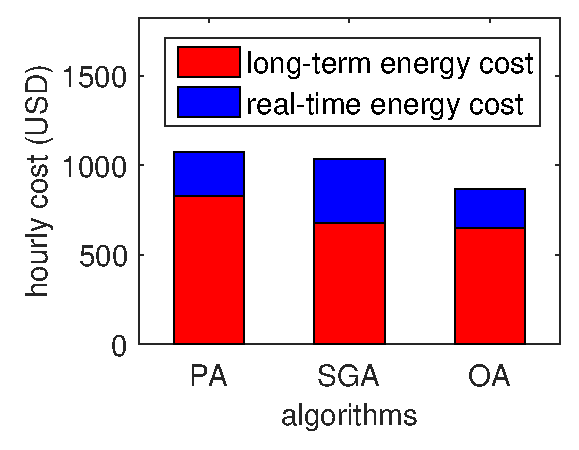
\includegraphics[width=0.9\linewidth]{figs/cost_comparison_beta_0}
	\caption{Cost comparison when $\beta=0$}
	\label{fig:cost_comparison_beta_0}
\end{figure}
\begin{figure}
\centering
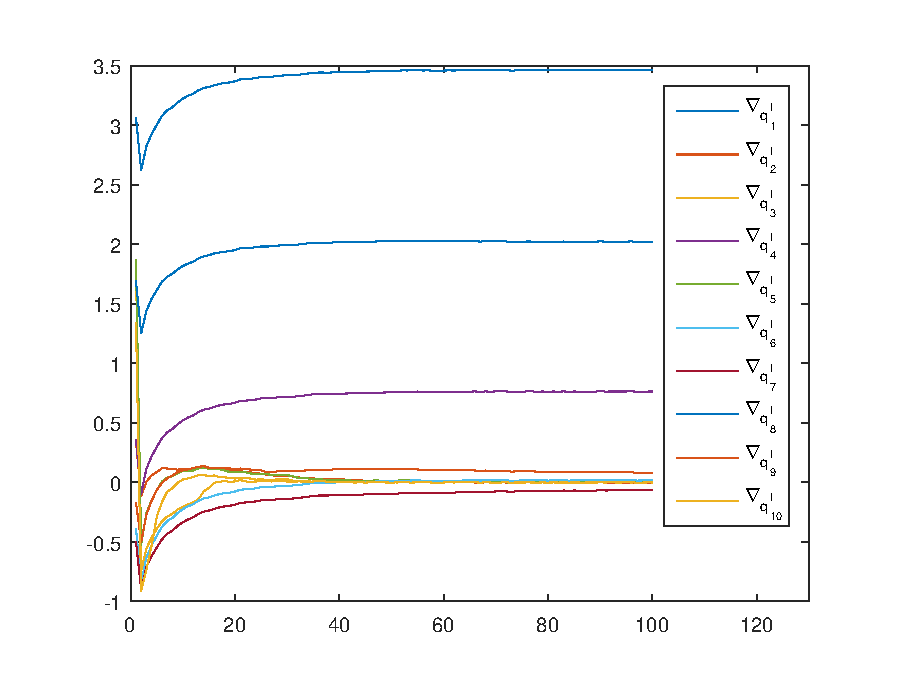
\includegraphics[width=0.9\linewidth]{figs/gradient_beta_0}
\caption{gradients}
\label{fig:gradient_beta_0}
\end{figure}

In Figure \ref{fig:cost_comparison_beta_0}, the system do not consider the queueing delay, i.e. $\beta=0$,
\begin{itemize}
	\item The gap between OA and PA is large
	\item However, the gap between PA and SGA is still small, why? 
\end{itemize}

There are some possible reasons why the gap between PA and SGA is small as

\begin{itemize}
	\item Is the number of samples large enough? Yes, it is in Figure \ref{fig:converge_debug}
	\item Is the algorithm convergent? Yes, it is.
	\item Because of GLB? Try with the single data center as in Figure \ref{fig:singleDC}.
\end{itemize}

\begin{figure}[!h]	
	\centering
	\subfloat[Error distributions ]{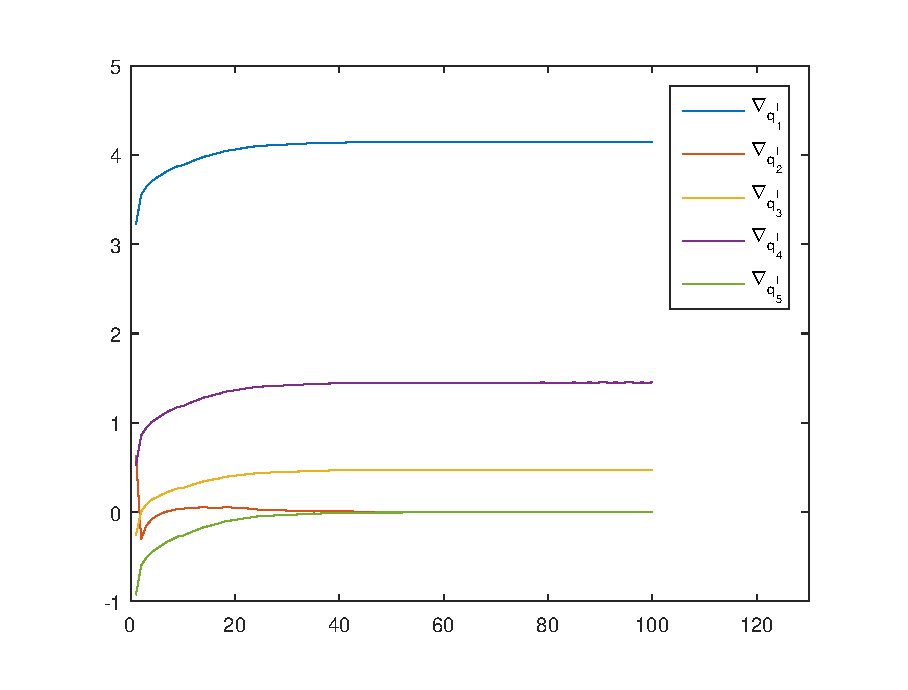
\includegraphics[width=.5\linewidth]{figs/grad_five_dcs}}
	\subfloat[Prediction errors ]{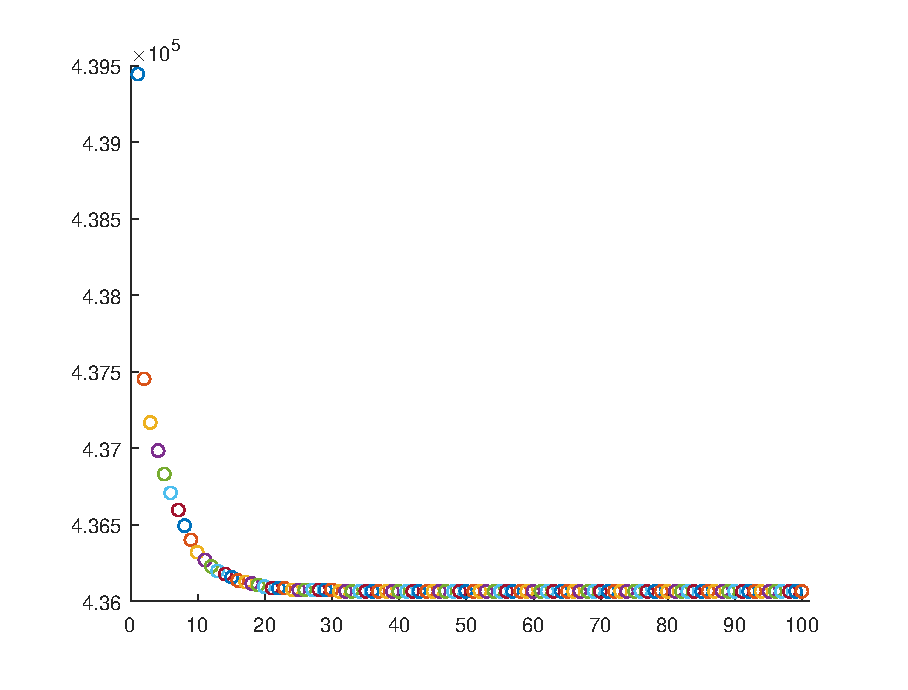
\includegraphics[width=.5\linewidth]{figs/grad_five_dcs_obj}}	
	\caption{Convergence with large number of samples (5 data centers).}
	\label{fig:converge_debug}
\end{figure}

\begin{figure}
	\centering
	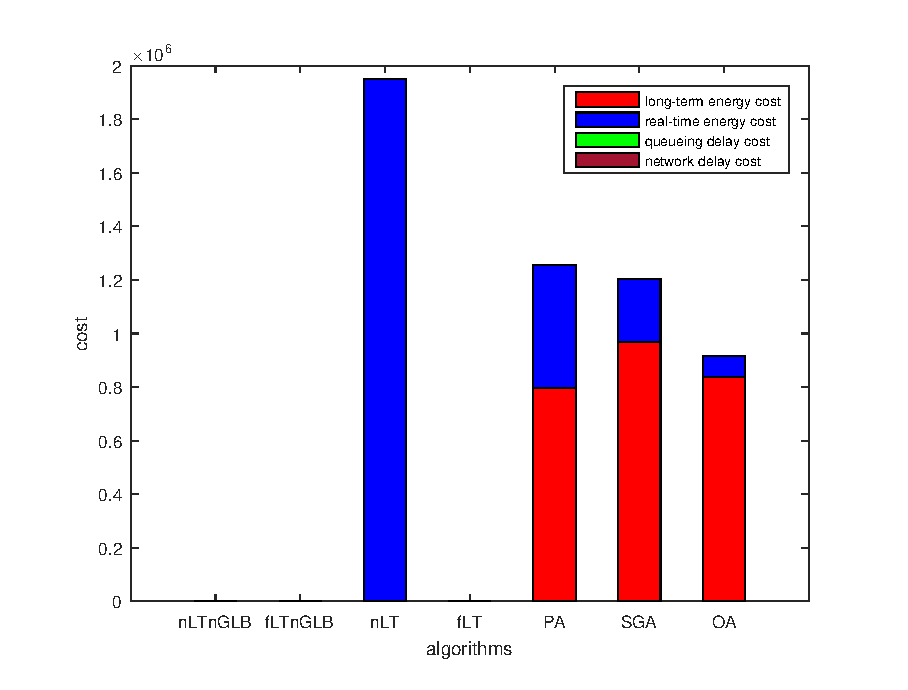
\includegraphics[width=0.9\linewidth]{figs/cost_comparison_single_dc_beta_zero}
	\caption{Single data center $\beta=0$}
	\label{fig:singleDC}
\end{figure}

